% (C) 2007/2008 Heiko Studt et al
%
% 2011 Martina Schacherbauer <tina.scha@yahoo.de>
% 2011 Simon Niechzial <simon@niechzial.de>
% 2011/2012 Sebastian Henneberg <henneber@fim.uni-passau.de>
% 2012 Manuel Grabowski <grabowski@fim.uni-passau.de>

%\documentclass[t,trans]{beamer}
\documentclass[t]{beamer}

\usepackage[utf8]{inputenc}
\usepackage{ngerman}
\usepackage{ifthen}
\usepackage[overlay,absolute]{textpos}
\usepackage{listings}
\usepackage{textcomp}

%\setbeameroption{show only notes}
%\setbeameroption{show notes on second screen}
%\setbeameroption{second mode text on second screen=right}

\usepackage{graphicx}
\title{Einführung in Android}
\author{Niko Fink, Marco Ziegaus}
\date{\today}

% \newcommand\killFSLogo{}
% \newcommand\bdashrule{}
\usetheme{IEEE}


\definecolor{javared}{rgb}{0.6,0,0} % for strings
\definecolor{javagreen}{rgb}{0.25,0.5,0.35} % comments
\definecolor{javapurple}{rgb}{0.5,0,0.35} % keywords
\definecolor{javadocblue}{rgb}{0.25,0.35,0.75} % javadoc
 
\lstset{language=Java,
basicstyle=\ttfamily,
keywordstyle=\color{javapurple}\bfseries,
stringstyle=\color{javared},
commentstyle=\color{javagreen},
morecomment=[s][\color{javadocblue}]{/**}{*/},
tabsize=4,
keepspaces,
showspaces=false,
showstringspaces=false}

%%%%%%%%%%%%%%%%%%%%%%%%%%%%%%%%%%%%%%%%%%%%%%%%%%%%%%%%%%%%%%%%%%%%%%%%%%%%%%%






%%%%%%%%%%%%%%%%%%%%%%%%%%%%%%%%%%%%%%%%%%%%%%%%%%%%%%%%%%%%%%%%%%%%%%%%%%%%%%%
\begin{document}

% TODO: Evtl. alternativ als erste Folie irgendwelchen hübschen Source-Code
% TODO: Nach Möglichkeit ohne Header usw.
\frame[plain, c]{
  \begin{center}
    \includegraphics[width=0.8\textheight]{pictures/Android_robot.png}
  \end{center}
}


\frame[plain,label=titel]{\titlepage}


\frame{
  \frametitle{Beispielslide}
  \vspace{5mm}
  \begin{itemize}
    \item foo
    \item bar
    \item foobar
    \item asdf
    \item qwerty
  \end{itemize}
}

\section{Einf\"uhrung}
\frame{
	\frametitle{Einführung}
	\vspace{5mm}
	\begin{itemize}
		\item weltweiter Marktanteil: 85 \%
		\vspace{2mm}
		\item Linux-Kernel
		\vspace{2mm}
		\item open source
		\vspace{2mm}
		\item Java (Logik) \& XML (GUI)
	\end{itemize}
}
	% führendes Betriebssystem für Smartphones
	% weltweiter Marktanteil ~85 \%
	% open source
	% Programmierung in Java (Logik) und XML (GUI, ähnlich wie JavaFX, C# mit XAML, etc.)

\frame{
	\frametitle{Versionen}
	\vspace{5mm}
	\begin{itemize}
		\item 2.3 (Gingerbread)
		\vspace{2mm}
		\item 3.0 (Honeycomb)
		\vspace{2mm}
		\item 4.0 (Ice Cream Sandwich)
		\vspace{2mm}
		\item 5.1 (Lollipop) --> aktuell
	\end{itemize}
}
	% Versionen
	% gut benutzbar seit 2.3.4 (Gingerbread, 2011)
	% seit 3.0 (Honeycomb) Tablet-Support
	% seit 4.0 (Ice Cream Sandwich) viele neue Möglichkeiten, z.B. Fragments
	% --> Seitdem Probleme mit älteren Versionen, Support Libraries
	% aktuell Version 5.1 (Lollipop) --> API-Level 22

\frame{
	\frametitle{Demo-App}
	\vspace{5mm}
	\begin{block}{Wetter am aktuellen Ort}
		\begin{itemize}
			\item GUI
			\vspace{2mm}
			\item GPS
			\vspace{2mm}
			\item Internet (openweathermap.org)
		\end{itemize}
		\vspace{5mm}
		\( \implies \) reduziert auf Minimal-Anforderungen
	\end{block}
}

	% Android als Framework, nicht als Library --> Inversion of control
	% Beispiel-App (reduziert auf Minimal-Anforderungen, ohne (vorerst) unnötigen Ballast), etc.

\section{App Komponenten}
\frame{
	\frametitle{Activities}
	TODO
}

% Bild einer (Sport-)Aktivität

\begin{frame}[c,fragile]
	\frametitle{Swing Button App}
	\begin{lstlisting}
	public static void main(String[] args) {
	    JFrame myFrame = new JFrame();
	    myFrame.addComponent(
	        new JButton("Click me!"));
	    myFrame.show();
	    ...
	}
	\end{lstlisting}
	\pause \vspace{0.5cm}
	\begin{figure}
	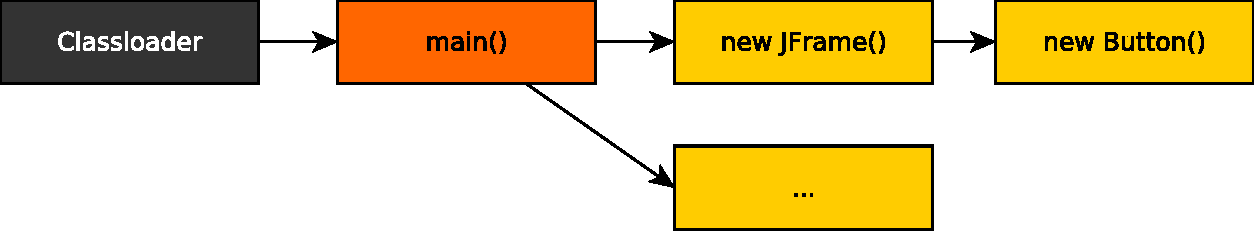
\includegraphics[width=\textwidth]{pictures/call-hierchy-swing.pdf}
	\end{figure}
\end{frame}

\frame[t]{
	\frametitle{Activities}
	% TODO Niko: Graphik MVC <-> Activity - Service - Content Provider + Intents + Broadcast Receiver
	\begin{itemize}
		\item View: Activity
		\item Controller: Service
		\item (Model: Content Provider)
		\item Kommunikation: Intents
		\item Listener: BroadcastReceiver
	\end{itemize}
}

\begin{frame}[c,fragile]
	\frametitle{Android Button App}
	\begin{lstlisting}[language=XML]
	<manifest>
	  <application label="ButtonApp">
	    <activity name=".MainActivity" 
	              label="Main Activity">
        ...
	</...>
	\end{lstlisting}
	\pause \vspace{0.5cm}
	\begin{lstlisting}
	class MainActivity extends Activity {
	    @Override
	    public void onCreate() {
	        //TODO add Button
	    }
	}
	\end{lstlisting}
\end{frame}

\frame[t]{
	\frametitle{Inversion of control}
	\centering
	\vspace{-0.2cm}
	\textbf{Swing}
	\begin{figure}
	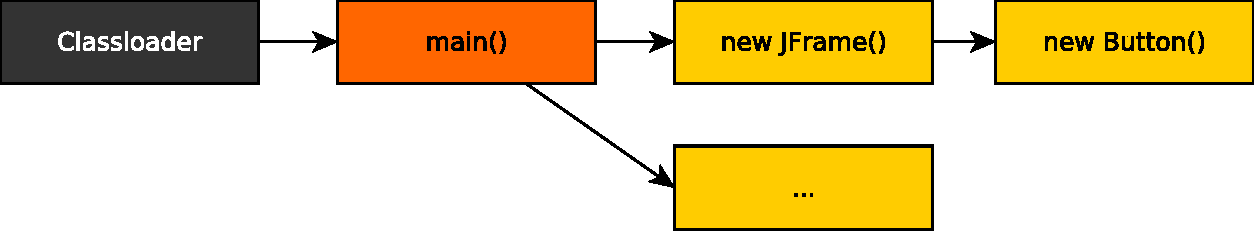
\includegraphics[width=0.8\textwidth]{pictures/call-hierchy-swing.pdf}
	\end{figure}
	\vspace{0.5cm}
	\textbf{Android}
	\begin{figure}
	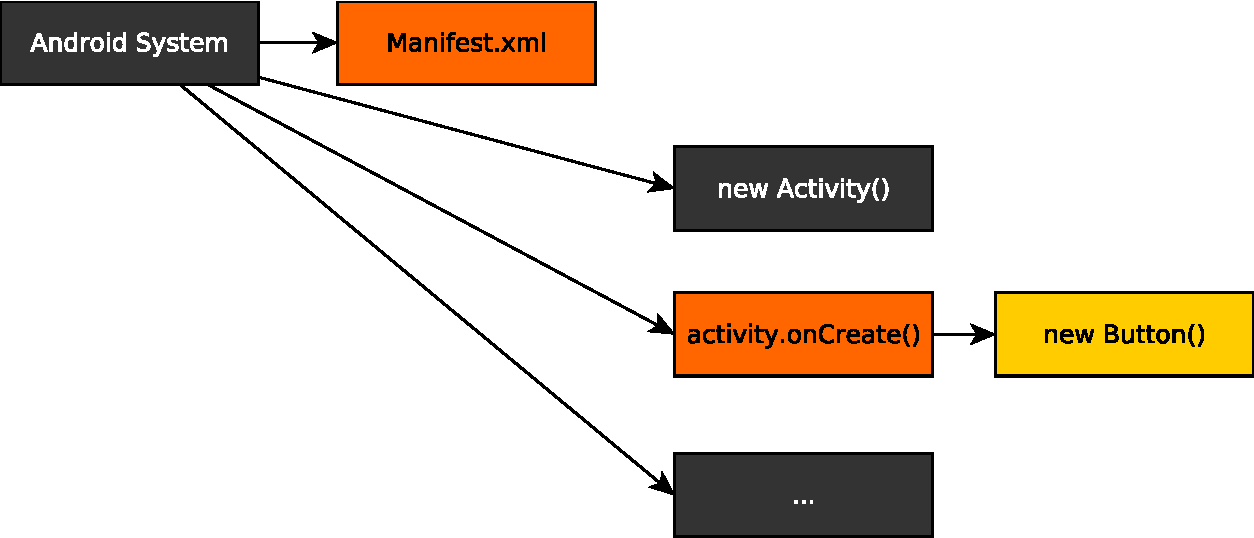
\includegraphics[width=0.8\textwidth]{pictures/call-hierchy-android.pdf}
	\end{figure}
}

\frame[c]{
	\frametitle{Activity Lifecycle}
	\begin{figure}
	\centering
	\includegraphics[width=\textwidth]{pictures/activity_lifecycle.png}
	\end{figure}
}

\frame[t]{
	\frametitle{Komponenten einer App}
	% TODO Niko: Graphik MVC <-> Activity - Service - Content Provider + Intents + Broadcast Receiver
	\begin{itemize}
		\item View: Activity
		\item Controller: Service
		\item (Model: Content Provider)
		\item Kommunikation: Intents
		\item Listener: BroadcastReceiver
	\end{itemize}
}

\frame[t]{
	\frametitle{Intents}
	% TODO Niko: intens als kommunikationsmittel in der App und zwischen apps
}
\section{GUI}
\frame{
	\frametitle{GUI}
	TODO
	% Übertriebenes Klickibunti-Bild
	% GUI wird in XML definiert
	% In Java holt man sich Referenzen darauf und kann es dann manipulieren
	% Layouts:
		% LinearLayout
		% TableLayout
		% RelativeLayout
}
\section{Sensoren}
\frame{
	\frametitle{Sensoren} \pause
	\vspace{5mm}
	\begin{itemize}
		\item Physikalisch:
		\begin{itemize} 
			\item GPS
			\vspace{2mm}
			\item Accelerometer/Beschleunigung
			\vspace{2mm}
			\item Helligkeit
			\vspace{2mm}
			\item Mikrofon	
		\end{itemize}
		\vspace{3mm}
		\item Virtuell:
		\begin{itemize} 
			\item Schrittzähler
			\vspace{2mm}
			\item Lineare Beschleunigung
			\vspace{2mm}
			\item Lage/Rotation
		\end{itemize}
	\end{itemize}
}

\begin{frame}[c,fragile]
	\frametitle{GPS}
	\vspace{-3mm}
	\begin{lstlisting}[language=Java]
		LocationListener listener;
		listener = new LocationListener() {
		    public void onLocationChanged(Location loc){
		    	// fetch the weather using the provided
		    	// location
		        fetchWeather(loc.getLatitude(),
		            loc.getLongitude()); 
		    }

		    public void onStatusChanged(...) {...}
		    public void onProviderEnabled(...) {...}
		    public void onProviderDisabled(...) {...}
		};
    \end{lstlisting}	
	
\end{frame}

\begin{frame}[c,fragile]
	\frametitle{GPS}
	\begin{lstlisting}[language=Java]
		// get a location manager
		LocationManager locationManager =
		    (LocationManager) getSystemService(
		        LOCATION_SERVICE);

		// request a single location update
		locationManager.requestSingleUpdate(
		    LocationManager.GPS_PROVIDER, listener,
		        getMainLooper());
		// getMainLooper() used for executing the
		// callback (ignore for now)
    \end{lstlisting}
\end{frame}

\begin{frame}[c,fragile]
	\frametitle{GPS}
	\begin{lstlisting}[language=Java]
		// request continuous location updates each
		// hour with a minimum distance of 1 km 
		locationManager.requestLocationUpdates(
		    LocationManager.GPS_PROVIDER,
		        1 * 60 * 60 * 1000, 1000, listener);
    \end{lstlisting}
    \pause
	\begin{lstlisting}[language=Java]
		// just get the last known location
		Location location = locationManager.
		    getLastKnownLocation(
		        LocationManager.PASSIVE_PROVIDER);
    \end{lstlisting}    
\end{frame}

\begin{frame}[c]
	\frametitle{Darf ich das?}
	\pause
	\begin{center}
		\includegraphics[width=8cm]{pictures/permissions.png}
	\end{center}
\end{frame}

\begin{frame}[c,fragile]
	\frametitle{Ja!}
	\begin{lstlisting}[language=XML]
		<uses-permission android:name=
		    "android.permission.ACCESS_FINE_LOCATION" />
		<uses-permission android:name=
		    "android.permission.ACCESS_NETWORK_STATE" />
		<uses-permission android:name=
		    "android.permission.INTERNET" />
	\end{lstlisting}
\end{frame}






\section{Threading}
\frame[t]{
	\frametitle{Threading Problems}
	\begin{figure}
	\includegraphics[width=\textwidth]<1>{pictures/errors-1.png}
	\includegraphics[width=\textwidth]<2>{pictures/errors-2.png}
	\includegraphics[width=\textwidth]<3>{pictures/errors-3.png}
	\end{figure}
}

\frame[c]{
	\frametitle{Android Threading}
	\begin{itemize}
	\item \textbf{Android UIs sind single-threaded!} \pause
	\item länger laufende Tasks auf dem UI Thread blockieren die App \\
		$\Rightarrow$ \emph{App-Not-Responding} Dialog wird angezeigt \pause
	\item IO ist im UI Thread verboten \\
		$\Rightarrow$ sonst \texttt{NetworkOnMainThreadException} \pause
	\item UI kann nur vom UI Thread aus aktualisiert werden  \\
		$\Rightarrow$ sonst \texttt{CalledFromWrongThreadException} \pause
	\item Threads, die von einer Activity aus gestartet wurden, \\ werden beendet sobald die Acitvity geschlossen wird \pause
	\item Activities (und damit auch alle Threads) werden neu gestartet, \\ wenn der Bildschirm gedreht wird
	\end{itemize}
}

\frame[c]{
	\frametitle{Alternativen}
	\begin{itemize}
	\item Starte anderen Thread und aktualisiere UI mit \texttt{Activity.runOnUiThread(Runnable)} \\ \pause
		$\Rightarrow$ \emph{Kommunikation mit UI trotzdem sehr aufwändig}\pause
	\item Verwende \texttt{AsyncTask}  \pause
		\begin{itemize}
		\item \texttt{onPre/PostExecute()} auf dem UI Thread \pause
		\item \texttt{doInBackground(...)} asynchron \pause
		\item Parameter und Rückgabewerte \pause
		\item Fortschritt mit \texttt{onProgressUpdate(...)} \pause
		\item Abbrechen mit \texttt{cancel()} \pause
		\end{itemize}
		$\Rightarrow$ \emph{wird immernoch zusammen mit Activity beendet}
	\end{itemize}
}

\begin{frame}[c]
	\frametitle{Services}
	\begin{itemize}
	\item Eigenständige Komponente neben Activities \pause
	\item läuft über längere Zeit im Hintergrund \pause
	\item asynchron und unabhängig von Activities \pause
	\item Aufgabenbereiche
		\begin{itemize}
		\item Dateiup- und download \pause
		\item Datensynchronisierung \pause
		\item Notifications \pause
		\item Datenlogging \pause
		\item Zeitgesteuerte Abläufe
		\item ...
		\end{itemize}
	\end{itemize}
\end{frame}

\begin{frame}[t]
	\frametitle{Arten von Services}
	\begin{itemize}
	\item \textbf{IntentService}
		\begin{itemize}
		\item Arbeitspakete in Form von Intents \pause
		\item arbeitet der Reihe nach ab und beendet sich automatisch \pause
		\item Wertrückgabe in Form von Intents \pause
		\end{itemize}

	\item \textbf{Started Service}
		\begin{itemize}
		\item durch Intent(s) gestartet \pause
		\item unbeschränkte Lebensdauer \pause
		\end{itemize}

	\item \textbf{Bound Service}
		\begin{itemize}
		\item hält Verbindung mit Activities, mit diesen direkte Kommunikation \pause
		\item Lebenszeit an die der Activities gebunden
		\end{itemize}
	\end{itemize}
\end{frame}




% \frame{
%   \frametitle{Ablauf}
%   \tableofcontents
% }

% \include{begruessung}
% \include{fachschaft}
% \include{Quitschie}
% \include{tipps}
% \include{lageplan}
% \include{tueten}


\end{document}